\chapter{Introduction Générale}

\section{Contexte et problème}

Depuis toujours l'homme a mis au point des techniques et méthodes pour exploiter les plantes afin de produire des médicaments.
De nos jours pour prévenir des maladies ou en guérir, nous utilisons des médicaments spécifiques obtenus en laboratoire par expérimentations d'essaies-erreurs sur ces produits naturels, pour en déceler et en extirper les principes actifs qui leur permettent d'avoir des effets sur les parasites ou virus qui conduisent à ces maladies.
On peut parler de l'Artémisine contenu dans l'Artemisia qui réagit nocivement sur le plasmodium, qui est la source du paludisme, maladie la plus fréquente à l'heure actuelle dans nos localités.

L’avenue d’Internet et des nouvelles technologies physico-chimiques, ont permis de voir affluer de grande quantité de données chimiques et biologiques de principes actifs et autres molécules, qui ont pu pour certaines, être accessibles au grand public.
Cette grande quantité de données contenus dans des bases de données telque MedChem \footnote{Site officiel de MedChem \href{https://www.medchem.be/}{https://www.medchem.be/}}, NIST \footnote{Site officiel de NIST \href{https://www.nist.gov/srd/nist-standard-reference-database-1a}{https://www.nist.gov/srd/nist-standard-reference-database-1a}} , MetaSpace \footnote{ Site officiel de MetaSpace \href{https://metaspace2020.eu/}{https://metaspace2020.eu/}}, MassBank \footnote{Site officiel de MASSBANK \href{https://massbank.eu/MassBank/}{https://massbank.eu/MassBank/}}, ReSpect \footnote{Site officiel de ReSpect \href{https://respectem.com/?page_id=42}{https://respectem.com/?page\_id=42}}, ont permis de voir émerger plusieurs outils et techniques afin de les exploiter pour optimiser les processus expérimentaux. On peut citer des méthodes d'apprentissage artificielle \cite{saldivar2022natural} (Machin Learning) qui visent, à identifier les molécules réagissant sur les parasites de maladies spécifiques en utilisant des modèles de classification, à prédire les fonctions biologiques de molécules tels que la bio-activité par rapport à un ensemble de parasites ou molécules spécifiques grâce à des modèles de prédiction, à générer des structures de molécules qui pourraient être des constituants de principes actifs contre des parasites donnés grâce à des modèles de génération.
%Par leur défaut de se spécifier sur des maladies spécifiques, ces méthodes sont peu exploités pour les quantités des données accessibles et peu inclusives dans des cas d'utilisation globale comme la recherche exploratoire de molécules,
On retrouve aussi des outils qui visent à exploiter plus généralement les données par exploration, à savoir Sherlock \cite{wenk2023sherlock}, LOTUS \cite{rutz2021lotus}, ENPKG \cite{gaudry2023sample} qui permettent l'élucidation de structures de molécules bioactives ou non, qui utilisent comme représentations des molécules les spectres MS et RMN qui contiennent des informations obtenues de leurs structures dans des états données (ionisation, excitation).

Dans le cadre de la recherche de molécules basée sur les produits naturelles, les biologistes utilisent de nos jours des outils tels que GNPS \cite{wang2016sharing} et MADByTE \cite{egan2021development}, qui exploitent les spectres MS ou RMN des molécules à explorer.
Ils ont pour but de produire des réseaux ou encore carte de ces molécules qui regroupent celles qui sont similaires entre eux, contenant leurs spectres et leurs structures (pour celles qui sont identifiées) en métadonnées.
Ces réseaux appelés réseaux moléculaires sont grandement utiles car permettent de détecter des similitudes entre molécules pour orienter les expérimentations d'essais-erreurs qui sont longues.
Néanmoins malgré le fait que l'on sache que les spectres MS et RMN contiennent des informations complémentaires issus des constituants des molécules, à notre connaissance aucune méthode existante ne permet de les exploiter simultanément, que ce soit les modèles de prédiction, classification et de génération.

\section{Question de recherche}
L'objectif du travail de recherche effectué dans le cadre de ce mémoire est de répondre à la question suivante:
Comment exploiter la complémentarité des spectres MS et RMN dans le but d'orienter et d'accélérer les expérimentations de découverte de molécules, basée sur les produits naturels, qui conduisent à identifier des réseaux moléculaires?

Pour répondre à cette question, nous proposons deux méthodes basées sur les techniques d'apprentissage par ensemble Bagging et Boosting. L'idée principale de ces méthodes est d'utiliser GNPS et MADByTE (qui construisent des graphes de molécules identifiées ou pas sur la base de spectres MS et RMN respectivement), conjointement avec des algorithmes de clustering multi-vues MCLES ou MVGL. Pour introduire GNPS et MADByTE dans les apprentissages, nous utilisons l'algorithme DBSCAN qui va extraire les clusters contenus dans les réseaux moléculaires fournis par ces derniers, en définissant le voisinage d'une molécule dans un réseau.

\section{Généralités}
\subsection{Atome et Molécule}
    Tout élément dans la nature est constitué de particules de très petites tailles qu'on appelle \textbf{atomes}.
    On peut citer les atomes de produits organiques suivants: le carbone (C), l'hydrogène (H), l'oxygène (O) et l'azote (N).
    Ces atomes associés ou encore liés permettent d'avoir des \textbf{structures} dite de simple à complexe (grâce à des liaisons simples, doubles, triples, cycles), représentant des matières qu'on appelle des \textbf{molécules}.
    Ce sont donc ces molécules de taille éventuellement grande ou petite qui forment la matière.
    Il existe de ce fait des molécules capables de guérir des maladies, par le biais de leur capacité d'initier des suites de réactions.
    On appelle ces molécules des molécules bio-actives; “bio” parce qu'elles participent aux réactions internes (métabolisme) et à l'entretien d'un organisme vivant et “actives” pour leur capacité à déclencher des réactions chimiques sur d'autres molécules précises.

    Dans le cadre des recherches visant à concevoir des médicaments en s’appuyant sur les produits naturels, les biologistes réalisent un ensemble d'étapes expérimentales \cite{nothias2018bioactivity} sur pour identifier les molécules bio-actives y contenus.
    On peut citer comme exemple l'Artemisia qui permet d'agir nocivement sur le plasmodium (parasite causant le paludisme), ou encore l'hoffe (l'igname bulbifère) qui a des propriétés de défense (anti oxydantes).
    Ces étapes bien qu'elles ont permis de trouver des ensembles de molécules bio-actives, dégradent ou détruisent malheureusement les molécules qui entrent dans le processus.
    De plus, ils détruisent parfois des synergies entre ces molécules qui permettaient d’observer leurs activités.
    
    Pour réduire ces effets, les biologistes exploitent les molécules déjà \textbf{identifiées} en laboratoire, pour faciliter l'identification de celles inconnues.
    Ils sauvegardent ainsi dans des bases de données spécifiques, leurs métadonnées constituées de leurs structures contenues dans leurs représentations \acrshort{SMILE} et \acrshort{INCHI}, avec d'autres à savoir leurs spectres MS(\acrlong{MS}) ou RMN(\acrlong{RMN}).
    Les spectres {MS} et {RMN} (et autres), ne sont pas utilisés de façon anodine car en pratique il y'a plus de difficulté à obtenir des structures de molécules par expérimentations, que d'avoir leurs spectres.
    D'où l'utilisation de techniques de spectrométrie.
    
    \subsection{Spectrométrie}

    La \textbf{spectrométrie} est une discipline qui visent à obtenir des grandeurs physiques d'éléments donnés, qui sont dans notre cas des molécules.
	Elle permet d'avoir par le biais de ces grandeurs, un ensemble d'informations issues des structures des molécules.
    
    Des informations qu'on souhaite extrairent, on retrouve plusieurs types de spectrométrie à l'instar de la \textbf{spectrométrie de masse} (\acrshort{MS}), la \textbf{spectrométrie par résonance magnétique nucléaire} ( \acrshort{RMN}) et de la spectroscopie infrarouge (\acrshort{IR}), etc \dots.
    En biologie ceux qui sont les plus utilisés sont les spectrométrie de masse et par résonance magnétique nucléaire.

    \subsubsection{Spectrométrie MS}
    Cette méthode de spectrométrie a pour but d'extraire d'un élément chimique, la masse sur charge et l'abondance relative de ses fragments de molécules ionisés appelés couramment radicaux \footnote{ Lien du site d'explication \href{https://www.studysmarter.fr/resumes/physique-chimie/chimie/spectrometrie-de-masse}{https://www.studysmarter.fr/resumes/physique-chimie/chimie/spectrometrie-de-masse}} \cite{menet2011principes}.
    Ces informations constituent ce qu'on appèle un spectre de masse ou spectre  \acrshort{MS}, qu'on visualise généralement sur un graphique semblable à celui de la Figure \ref{fig:ms_glycerol} \footnote{Prise sur \href{https://www.chemicalbook.com/SpectrumEN_56-81-5_Raman.htm}{https://www.chemicalbook.com/SpectrumEN\_56-81-5\_Raman.htm}} correspondant à celui du glycérol contenu généralement dans les cirots prescrits dans des formations sanitaires.
    
    \begin{figure}
   	 \centering
   	 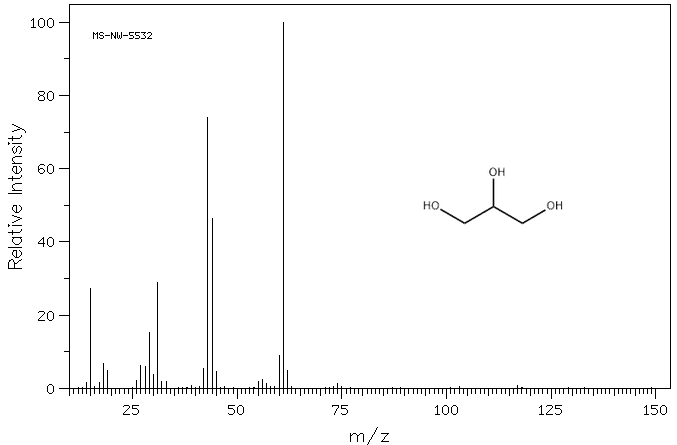
\includegraphics[width = 0.7\linewidth]{Images/ms_glycerol.png}
   	 \caption{Spectre MS du Glycérol}
   	 \label{fig:ms_glycerol}
    \end{figure}
    
    Pour pouvoir le faire on utilise une machine spécialisée appelée spectromètre de masse qui contient généralement :
    \begin{itemize}
   	 \item un tube de liquide : dans lequel on introduit l'élément chimique
   	 \item un ioniseur : qui par le biais de faisceau d'électrons permet d'ioniser l'élément
   	 \item un accélérateur de particules : qui a pour but de dévier les radicaux d'un rayon de courbure qui dépend de leur masse sur charge
   	 \item un détecteur : qui permet d'évaluer ces rayons de courbure (par conséquent les masses sur charge) et d'avoir les abondances de ces radicaux (ou encore intensité)
    \end{itemize}
    
    On parle ainsi de :
    \begin{itemize}
   	 \item Spectrométrie de masse à haute résolution \acrshort{HRMS}:
   	 lorsqu'on utilise des spectromètres de masse spécialisés tels que \textbf{Orbitrap}.
   	 \item Chromatographie liquide/ Spectrométrie de masse \textbf{LC/MS}:
   	 lorsqu'on utilise la technique de séparation de molécules contenues dans une solution aqueuse nommée chromographie avant la spectrométrie de masse  
   	 \item Spectrométrie \textbf{$MS^{2}$} (MS/MS) :
   	 lorsqu'on utilise des spectromètres de masse qui possèdent deux étapes d'ionisation consécutives avant analysation
    \end{itemize}

    \subsubsection{Spectrométrie RMN}

    Cette méthode de spectrométrie a plutôt pour but d'extraire d'un élément chimique, les déplacements chimiques et les intensités d'excitation que réalisent ses atomes de types spécifiques (Hydrogène, Carbone etc \dots), lorsqu'il est placé dans un champ magnétique (zone de forces issues d'un aimant ou de déplacements d'électrons).
    Ces informations constituent ce qu'on appelle un spectre de résonnance magnétique nucléaire ou encore spectre  \acrshort{RMN}, qu'on visualise généralement sur un graphique semblabe à celui de la Figure \ref{fig:hrmn_glycerol} \footnote{Prise sur \href{https://www.chemicalbook.com/SpectrumEN_56-81-5_Raman.htm}{https://www.chemicalbook.com/SpectrumEN\_56-81-5\_Raman.htm}} étant celui du glycérol.

    \begin{figure}
   	 \centering
   	 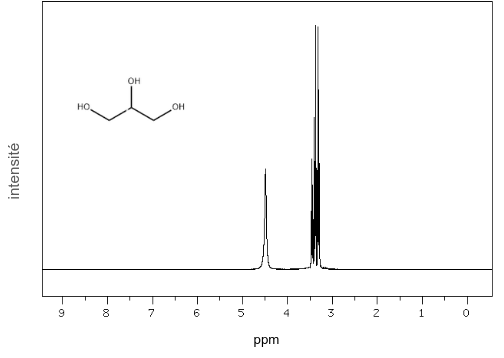
\includegraphics[width = 0.7\linewidth]{Images/hrmn_glycerol.png}
   	 \caption{Spectre RMN du Glycérol observant les atomes d'hydrogène}
   	 \label{fig:hrmn_glycerol}
    \end{figure}

    Pour obtenir ces informations, on utilise un spectromètre  \acrshort{RMN} encore appelé sonde RMN, qui est un compartiment qui permet d'utiliser des champs magnétiques excitant des types d'atomes précis d'une molécule, en considérant un champ de base (celui agissant sur le Tetramethylsilane TMS).

	 Lorsqu'on observe 'n' types d'atomes on parle de spectrométrie 'n-RMN', par exemple pour:
   	 \begin{itemize}
   		 \item la spectrométrie \textbf{1-RMN} : on a la spectrométrie sur hydrogène (H-RMN), Spectrométrie sur carbone (C-RMN)
   		 \item la spectrométrie \textbf{2-RMN} : on a  \acrfull{TOCSY} qui observe les croisements hydrogène-hydrogène), \acrfull{HSQC} qui observe les croisements hydrogène-carbone
   	 \end{itemize}

    Ces techniques permettent d'avoir des informations sur des molécules sans pour autant avoir leurs structures, qui en laboratoire est un processus long surtout pour la découverte de médicaments basée sur les produits naturels.
    Ils sont très utiles dans ce processus car ils permettent d'éviter de réaliser des expérimentations sur des molécules déjà identifiées en observant les correspondances de spectres entre molécules. On appelle cette opération la déréplication.
    
    \subsection{Déréplication et réseau moléculaire}

   	 La \textbf{déréplication} est une opération qui consiste à trouver dans un ensemble de molécules, celles qui ont déjà été identifiées par correspondance de spectres par rapport à celles identifiées et sauvegardées dans des bases de données.
   	 Elle permet de réduire les expérimentations d'essais - erreurs en donnant la possibilité de se concentrer sur des molécules inconnues.
   	 Dans le but de retrouver ces molécules inconnues, on observe leurs correspondances avec ceux qui ont été identifiées pour essayer de détecter les synergies et relations qui peuvent exister entre elles.
  	 
   	 Pour bien le visualiser, on utilise un graphe où un nœud correspond à une molécule (représentée par un spectre), avec une liaison entre deux nœuds correspondant au niveau de ressemblance (similarité) ou de différence entre eux.
   	 Il faut noter que ces nœuds ou encore sommets portent les métadonnées disponibles de leurs molécules correspondantes.
   	 On appelle ce type de graphe un \textbf{réseau moléculaire}, qui plus formellement est un graphe epsilon-voisinage, avec des sommets étant des molécules et des arêtes correspondant à la similarité ou la dissimilarité entre leurs spectres (\acrshort{MS} ou \acrshort{RMN}).
  	 
   	 Plus ce réseau contient de molécules identifiées, plus on augmente les possibilités d'identifier toutes les molécules y contenues par des restrictions d'expérimentation.
   	 On parle ainsi de \textbf{réseau identifié} quand toutes les molécules y contenues sont identifiées.
   	 Cela signifie que bien construire un réseau moléculaire (par le choix de métrique et des liaisons) permet d'accélérer le processus de découverte.
   	 Des différents moyens d'en construire et du type de spectre utilisé, il existe plusieurs outils ou méthodes dont les plus communs sont \acrfull{GNPS} et \acrfull{MADByTE}.
  	 
   	 \subsubsection{\acrfull{GNPS}}
  	 
   	 \textbf{GNPS} \cite{wang2016sharing} est une plateforme dont le processus principal prend en entrée des spectres MS de molécules pour construire le réseau moléculaire.
   	 Comme on peut le voir sur la Figure \ref{fig:gnps3}, ce processus suit plusieurs étapes:
  	 
   	 \begin{figure}
   		 \begin{center}
       		 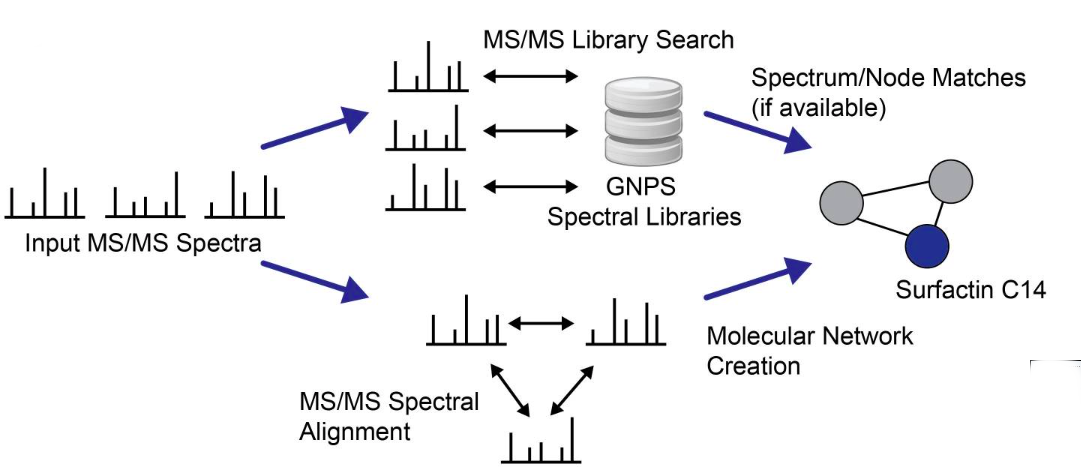
\includegraphics[width = 0.7\textwidth]{Images/GNPS4.png}
   		 \end{center}
   		 \caption{Processus de GNPS \cite{wang2016sharing}}
   		 \label{fig:gnps3}
   	 \end{figure}

   	 \begin{itemize}
   		 \item \textbf{Construction du template du réseau des molécules d'entrées} : cette étape a pour objectif de construire le réseau des molécules d'entrées en utilisant comme mesure de similarité le cosinus de similarité avec un seuil donné (plus de 0.63 en pratique)
   		 \item \textbf{Identification des molécules par correspondance dans sa base de données}  : cette étape à pour objectif de trouver les molécules d'entrées qui sont déjà dans la base de données, en faisant une recherche basée sur la correspondance de spectres utilisant le cosinus de similarité et également un seuil donné (plus de 0.7 en pratique)
   		 \item \textbf{Attachement des méta-données au template précédent}: cette étape visent à ajouter les informations des molécules identifiées et non identifiées sur leurs sommets respectifs du graphe.
   	 \end{itemize}

   	 Il faut noter que chacune des valeurs de seuil de similarité utilisées ont des significations particulières pour les biologistes. Si le seuil a une valeur supérieure à 0.7 alors on cherche des correspondances exactes, si par contre, on a une valeur comprise entre 0.63 à 0.7, on cherche des correspondances pour exploration.
  	 
   	 \subsubsection{\acrfull{MADByTE}}

   	 \textbf{MADByTE} est également un outil qui permet de construire le réseau moléculaire correspondant à un ensemble de spectres de molécules; il prend en entrée les spectres HSQC et TOCSY des molécules.
   	 Le réseau est tout de même différent qu'avec celui de GNPS, car on retrouve un nouveau type de nœud associé à un système de spin.
  	 Un système de spin est un ensemble de déplacements chimiques considérés comme identiques par tolérance.
   	 De ce fait, une molécule peut être vue comme un ensemble de systèmes de spins qu'il contient, et à cet effet son sommet est relié à tous ceux de ses systèmes de spins d'une similarité complète.

   	 Comme on peut le voir sur la Figure \ref{fig:madbyte}, ils suit les étapes suivantes:
   	 \begin{itemize}
   		 \item \textbf{Prétraitement des spectres \acrshort{HSQC} et \acrshort{TOCSY}} : cette étape vise à supprimer les déplacements considérés comme inutiles, en tenant compte des solvants qui ont été utilisés pour acquérir les spectres et en s'assurant qu'après suppression les spectres TOCSY soient toujours symétriques

   		 \item \textbf{Croisement des spectres TOCSY et HSQC obtenus} : cette étape vise à conserver les déplacements qui se correspondent par rapport aux atomes d'hydrogènes pour chacun des couples de spectres

   		 \item \textbf{Calcul des système de spins} : cette étape vise à regrouper les déplacements identiques que sont les systèmes de spins avec des marges d'erreur donnés pour les atomes d'hydrogène et de carbone

   		 \item \textbf{Construction du réseau}: cette étape vise à construire le réseau de molécules.
   		 On calcule les similarités entre les systèmes de spins en utilisant l'indice de Jaccard.
   		 Il faut aussi noter que chaque sommet d'une molécule sera lié aux sommets de tous ses systèmes de spins d'une valeur de similarité complète (valeur 1)
   	 \end{itemize}

   	 \begin{figure}
   		 \begin{center}
       		 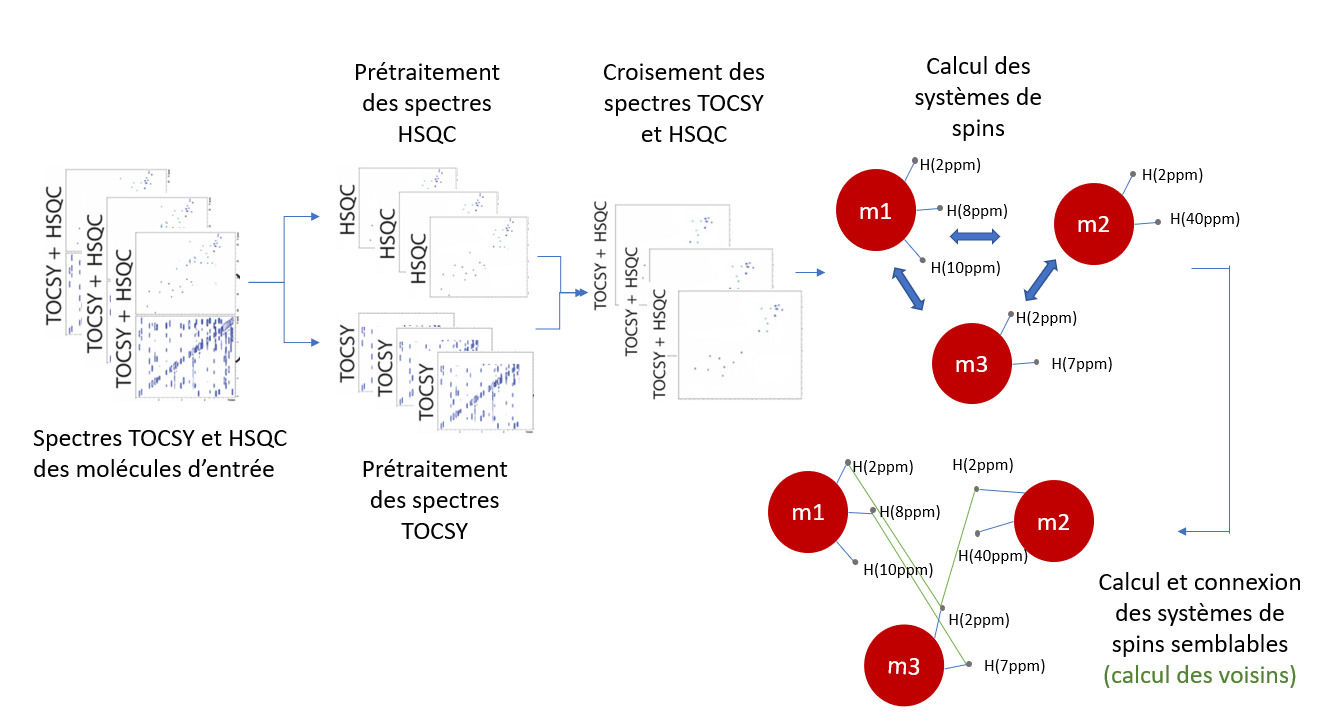
\includegraphics[width = 0.7\textwidth]{Images/madbyte.png}
   		 \end{center}
   		 \caption{Processus de MADByTE}
   		 \label{fig:madbyte}
   	 \end{figure}

   	 On obtient un réseau qui, pour des raisons de lisibilité peut être simplifié en supprimant les sommets de systèmes de spins qui ne sont liés à aucun autre système.
   	 On obtient un \textbf{réseau d'association} qui peut encore être plus lisible en considérant les sommets de systèmes de spins connectés comme un sommet.

   	 Nous remarquons que l'on utilise un réseau moléculaire parce qu'il permet d'explorer des liaisons entre les molécules, tout en regroupant les molécules ou encore spectres similaires dans des groupes ou encore clusters qui se forment naturellement.
   	 Ces groupes qu'on retrouvent permettent par le biais d'observations et d'analyse des spectres, et des structures des molécules identifiées, d'avoir des orientations d'expérimentations.
   	 De ce fait les algorithmes comme GNPS et MADByTE regroupent des spectres de molécules les plus semblables, ce qui se rapproche très clairement du clustering.

\section{Plan du mémoire}

Le reste de ce mémoire est organisé comme suit.
Le Chapitre 2 présente %les bases nécessaires à la compréhension du travail, allant des notions d'atomes et molécules aux réseaux moléculaires. Il se termine par
une revue de littérature des méthodes de clustering, de clustering multi-vues et d’ensemble de clustering utiles à la résolution du problème.
Dans le Chapitre 3, nous détaillons les méthodes proposées.
Le Chapitre 4 présente nos expérimentations et les résultats obtenus.
Enfin, le Chapitre 5 conclut ce document en résumant les principaux résultats et en discutant des implications futures de notre recherche.

